\section{Miscellaneous works} 
\label{sec:related}

Besides the major NVMM works we have introduced, 
there are NVMM systems designed from
different perspectives. For exmaple, some works rely more on hardware support
to reduce system overhead, and some focus on NVMM protection.
In this section we will talk about miscellaneous works
on NVMM system software design.

\subsection{Eliminate the consistency/atomicity overhead} 
\label{sec:systemdesign}

\begin{table}
	\resizebox{\linewidth}{!}{
	\footnotesize
	\centering
	\begin{tabular}{|l|c|c|c|c|c|}
	\hline
%	\multirow{4}{*}{}&PMFS &\DAChell{}\\\hline
%	&\multicolumn{2}{c|}{(Ops per second)}\\\hline
	System & In-place & Logging & COW & clflush & mfence\\\hline
	\hline
	BPFS & * & No & Yes & No & Yes  \\\hline
	PMFS & Yes & Yes & No & Yes & Yes  \\\hline
	Rio Vista & No & Yes & No & N/A & N/A  \\\hline
	Mnemosyne & * & Yes & Yes & Yes & Yes \\\hline
	NV-heaps & No & Yes & No & No & Yes  \\\hline
	CDDS & No & No & Yes & Yes & Yes  \\\hline
	UBJ & Yes & Yes & Yes & No & Yes  \\\hline
	eNVy & No & No & Yes & No & Yes  \\\hline
%	Kiln & Yes & No & No & No & No  \\\hline
	\hline
	Native & Yes & No & No & No & No  \\\hline
	\end{tabular}}
	\vspace*{1mm}
	\caption{\figtitle{Comparison of NVMM system software. * means in-place updates are only performed for memory stores to a single variable or at the granularity of cache line size. N/A means not specified in paper.}}
	\label{table:comparison}
\end{table}

Table~\ref{table:comparison} lists the mechanisms adoption status of some
systems we have introduced. Almost all the NVMM systems rely on logging or
copy-on-write to provide atomicity, and clflush and/or mfence to guarantee
consistency. Both of them add overhead to NVMM system software: logging doubles
the writes, copy-on-write amplifies the writes, and CPU cache flushing is
expensive~\cite{CPUcaching}. Some works eliminate the software overhead of
consistency and atomicity with hardware assistance.
\textbf{WrAP}~\cite{WrAP} avoids explicit CPU cache flushing by disabling
cache flushes to NVMM, and updates to the actual address are done by logging.

\textbf{Kiln}~\cite{Kiln} provides a persistent memory design
 that adopts a non-volatile
cache and a non-volatile main memory to enable atomic in-place updates without
logging or copy-on-write. Kiln moves the transaction commitment to the NV
cache layer, all the data are resided inside CPU cache (including last level
NV cache) before committed. When commit a transaction, Kiln flushes all
the dirty lines in volatile cache to NV cache, and then change the states of
NV cache lines to committed. Committed NV cache lines are persistent and
can be flushed to NVMM. Kiln has a similar programming interface as NV-Heaps
and Mnemosyne, but the majority contribution is the NV cache layer.

\textbf{WSP}~\cite{WSP} stands for whole-system persistence.
 It aims at systems where
all memory is NVMM, and it transparently recovers an application's entire state,
making a system failure appear as a suspend/resume event. WSP does not
do anything about logging or explicit CPU cache flushing; instead, it does 
\emph{flush-on-fail}, which flushes CPU registers and cache lines to NVMM
on system failure, using a small residual energy window provided by system
power supply. As WSP does not flush during normal operations, it eliminates
the runtime overhead of flushing CPU cache lines on each update entirely, also
it does not require any software modification such as NV-heaps~\cite{nvheaps}
 and Mnemosyne~\cite{mnemosyne}.

WSP consists of NVMM devices, a hardware power monitor, and software suspend/resume routines. When the WSP system fails, the hardware power monitor triggers
an interrupt to the CPU core. All the CPU cores flush their cache lines to the 
NVMM and then halts. On the recovery, resume routine does the inverse to recover
the system to the consistent state. As WSP eliminates the runtime persistency
operations, it shows good performance comparing to NV-heaps.

\ignore{
Some works give a overview of NVMM system and proposes software
design suggestions.
Bailey et al.~\cite{systemimplications} shows the implications for a NVMM-only
system. It addresses several changes and challenges to current system design,
such as paging and application running model. A NVMM-only system may benefit
from the persistency of NVMM for fast recovery, but also meets the security
and privacy issue which current system does not have. How to design a
NVMM-only system is still in exploration. Trivedi et al.\cite{onestack}
 examines the
properties of high-performance networking software stacks such as efficient
hardware access, operating system bypass and zero copy data movement,
points out that the I/O stack for NVMM should leverage from the mature and
stable networking stack, and proposes an unified I/O stack that deal with
network, local NVMM and remote NVMM under a common framework.
}

\ignore{
\subsection{Hardware/Software co-design} 
\label{sec:hwswdesign}

Most NVMM systems rely on some hardware primitives assistance, 
such as BPFS and PMFS.
However, they try to minimize the hardware modifications and resolves the
atomicity and consistency problems with software solutions,
such as explicit CPU cache flushing and logging.
Some researches try to leverage more hardware
solutions and make the software simple and efficient.

\textbf{WrAP}~\cite{WrAP} proposes a system architecture
 that provides persistence
ordering, persistence atomicity and persistence protection guarantees. 
WrAP keeps a log of update operations, but the key change is 
a victim persistence cache (VPC).

Every write to NVMM in WrAP results in two update paths: an atomic update to
the log area in NVMM, and a normal store instruction to the NVMM address. Both
paths are performed simultaneously. VPC holds PCM entries that are evicted
from the last-level cache, make sure they do not go to the actual address;
instead, the update to the home locations will be made
independently by copying the log entries.
By propagate the write operation in two paths, WrAP avoids the overhead of CPU
cache flushing.
\textbf{SoftWrap}~\cite{softWrAP}
 is the software implementation version of WrAP.
Instead of VPC, SoftWrAP installs a library
to transform applications to use the WrAP APIs to access the NVMM.
SoftWrAP
uses alias update, routes the cache entries to write to a different location
without affecting the original data. SoftWrAP achieves the same persistent
guarantee as WrAP without hardware modification, but not as efficient as WrAP.
}

\ignore{
\subsection{Recovery} 
\label{sec:recovery}

Several early researches focus on how to recovery the system with NVMMs.
\textbf{RVM}~\cite{RVM} is an efficient,
 portable and easily used implementation of
recoverable virtual memory for Unix enviorments. By eliminating the support
for nesting, distribution and concurrency control, the implementation of 
RVM becomes very simple and easy to use. RVM manages recoverable memory in
segments, each with a file or a disk partition as backing store. Applications
calls the interfaces provided by RVM to begin and commit transactions. RVM
uses a undo/redo logging strategy to make the persistency guarantee. 
}

\ignore{
A remaining issue of WSP is device recovery. As the device drivers are restored
-but the devices lost power and need to re-initialize, the state of software
-and hardware is not consistent. WSP proposes to clean up device state on
-the resume path, or virtualize the devices by using a VM hypervisor.
}

\subsection{Protection} 
\label{sec:protection}

As NVMM is sitting on the system memory bus and exposes the memory range
to the applications, how to protect it from stray writes become a issue.
\textbf{PMBD}~\cite{PMBD}
is an attempt to make a robust NVMM system free from stray writes.
PMBD treats NVMM as a block device sitting on the memory bus, as it is
easier to provide protection and order persistence for
a block device than a memory device.

PMBD proposes several solutions to protection and order persistence and
compare the performance. To enforce protection, one solution is to disable page
table entry for write until needed; however, this incurs big penalty on
TLB flush and performance is bad. Buffer the write requests and commit
them as a batch helps to improve the performance for sequential writes,
but not for random writes. The author finds out the best solution is 
\emph{private mapping}: NVMM pages are mapped to virtual space only when
required and unmapped after write finishes. Evaluation shows private
mapping provides 90\% bandwidth of the optimal case. Private mapping
addes overhead for each write request, but reduces page table size and
TLB pollution.

\ignore{
To guarantee write order, PMBD compares two solutions: use a non-temporal
store (\texttt{movntq}) to bypass the CPU cache and \texttt{sfence} to
flush the buffered data, or use \texttt{clflush} to flush CPU cache
and \texttt{mfence} to ensure the data is written back. With micro-benchmark
tests \texttt{movntq/sfence} generally works better than \texttt{clflush/mfence}
solution.
}

PMBD provides protection of NVMM with the cost of performance, as it appears
as a block device and cannot be accessed from user space directly.

\ignore{
The fact that
PMBD treats NVMM as a block device incurs significant overhead
as Linux block layer is designed for slow storage devices.
Also PMBD does not allow applications to access NVMM directly.
We don't think PMBD is the right solution to utilize NVMM, but it provides
some insights on NVMM protection, which is not addressed by system such as BPFS.
}

\ignore{
\textbf{CDSMM}~\cite{CDSMM} also presents the memory management module design
 for NVMMs.
Rather than performance, it focuses on security and protection: it introduces
techniques for 1) robust wear-aware memory allocation, 2) preventing for 
erroneous writes, and 3) consistency-perserving updates that are cache-efficient.

As hardware wear-leveling has performance issues, CDSMM presents a
software memory allocator that always allocate new blocks rather than reusing
old freed blocks to average the writes to each block. To reduce metadata
writes, CDSMM puts important information in DRAM and sync to NVMM only required.It also adds checksum to prevent stray writes from modifying metadata.
}

\textbf{CDSMM}~\cite{CDSMM} presents the MMU design for NVMMs, focuses on
security and protection. It protects NVMM pages with system call
\texttt{mprotect}, but performs it in a batch way so that to reduce mode
switch overhead, kernel structure modifying overhead and TLB flushes.
CDSMM also does a software wear-leveling by always allocating new blocks
rather than reusing old freed blocks to average the writes to each block.

The problem of CDSMM is that it adds significant overhead to software
programming.
CDSMM has several interesting ideas about NVMM protection, but
to integrate the design in applications is still difficult.

\ignore{
 To reduce metadata
cache line so that application can use command to track data is either in 
CPU cache or persistent on NVMM, and resolves the persistency and write ordering
issue. 

The disadvantage of CDSMM is that it requires both software and hardware
modifications, adds significant overhead to software programming. The paper
shows a B+ tree example and in order to apply CDSMM design, it does not only 
adds much more software efforts, but also change the definition of B+ tree:
the values in a node is not in sorted order and it takes linear time to search
value in a node. CDSMM has several interesting ideas about NVMM protection, but
to integrate the design in applications is still difficult.
}

\subsection{Wear leveling}
\label{sec:wear}
As NVMM has a lower endurance than DRAM, frequent writes will wear out
NVMM in a few years and makes it unusable. Without wear leveling, the lifetime
of a PCM based NVMM is just 0.5 to 3 years. This is unacceptable in a real
system. ~\cite{PCMHierarchy} introduces write line random shifting to uniform
the writes. ~\cite{PCM_EfficientMainMemory} tracks the redundant bit-writes to
eliminate the writes that do not change the value. It also uses byte-level row
shifting to rotate the writes at fine-grained granularity, as well as segment
swapping at coarse-grained granularity.

Implement wear leaveling in software has several disadvantages: first, it makes
the software more complex. Second, software needs additional space to store
the mapping data.
Also, each access to NVMM needs to check the mapping information, makes it
a performance bottleneck.
Third, Software wear leveling cannot be more efficient
than a hardware solution. We conclude that NVMM wear leveling should be
implemented in hardware. Start-Gap~\cite{startgap1} is a simple and effective
wear leveling technique for PCM-based NVMM. It uses only two registers and
makes NVMM robust to malicious attacks. \cite{secrefresh} and \cite{freep}
are another two hardware solutions to balance the writes to PCM and improve
lifetime.

\subsection{POSIX File Interface overhead}
\label{sec:noposix}

Most applications access the storage devices via POSIX interfaces, which are
designed to be general enough to apply for most cases, from file I/O
to network I/O.
This means, however, the POSIX-style file access functions are not optimized
for specific devices, and some of these are a poor match for NVMM.
In particular, the POSIX interface
requires the programmer to specify the buffer that \texttt{read()} copies data
to. POSIX places no constraints on the size
or alignment of the buffer, so a copy operation is usually unavoidable.  For
slow disks and even SSDs, the cost of this copy is small.
But for NVMM based system, the relative cost is much larger.
We test the latency of 4~kB read and
write operations of \DAChell{} with page table populated and page fault overhead
eliminated, and find out that the latency of memory copy to user buffer
accounts for 76\% for read and 77\% for write.
This high overhead of memory copying makes the POSIX interface
itself a major impediment to exploiting the performance of NVMM.

To eliminate it, we propose a new file read interface optimized for
NVMM-based storage systems.  The interface provides a new function:

\ignore{
\cfigure[Graphs/latency-break-quill.pdf,{\figtitle{Chell-Direct 4~kB read/write latency breakdown. Memory copy accounts for 76\% of total latency. Page table is populated on file open, so the page fault overhead is eliminated.}},fig:latency-break]
}

\vspace{1em}
\begin{tabular}{l}
ssize\_t \grb{}(int fd, char **buf, size\_t count);\\
%ssize\_t \gwb{}(int fd, char **buf, size\_t count);\\
\end{tabular}
\vspace{1em}

\ignore{How do writes work in this interface?  There's something missing here:  \gwb{} doesn't actually have any input data, right?  This gets me the address, but then I have to copy the data there, I guess.  That means I need to ensure that that memory won't go anywhere while I'm writing, and I need to make some other call to make sure that durability is ensured.  I think the best bet would be to just worry about reads, especially given the time remaining.}
\ignore{Yes. write is much more complicated.}

The interface is similar to the conventional \texttt{read}, except that calls
to \texttt{\grb{}} return a buffer to programmer via the \texttt{buf}
parameter.  The \texttt{*buf} contains a portion of the target file
(\texttt{fd}), starting from current file offset and extending for up to
\texttt{count} bytes.  The return value is the actual length of the memory
region.  No copying is necessary.  We added the \grb{} interfaces based to
\DAChell{}.

\ignore{
\begin{figure}[htb]
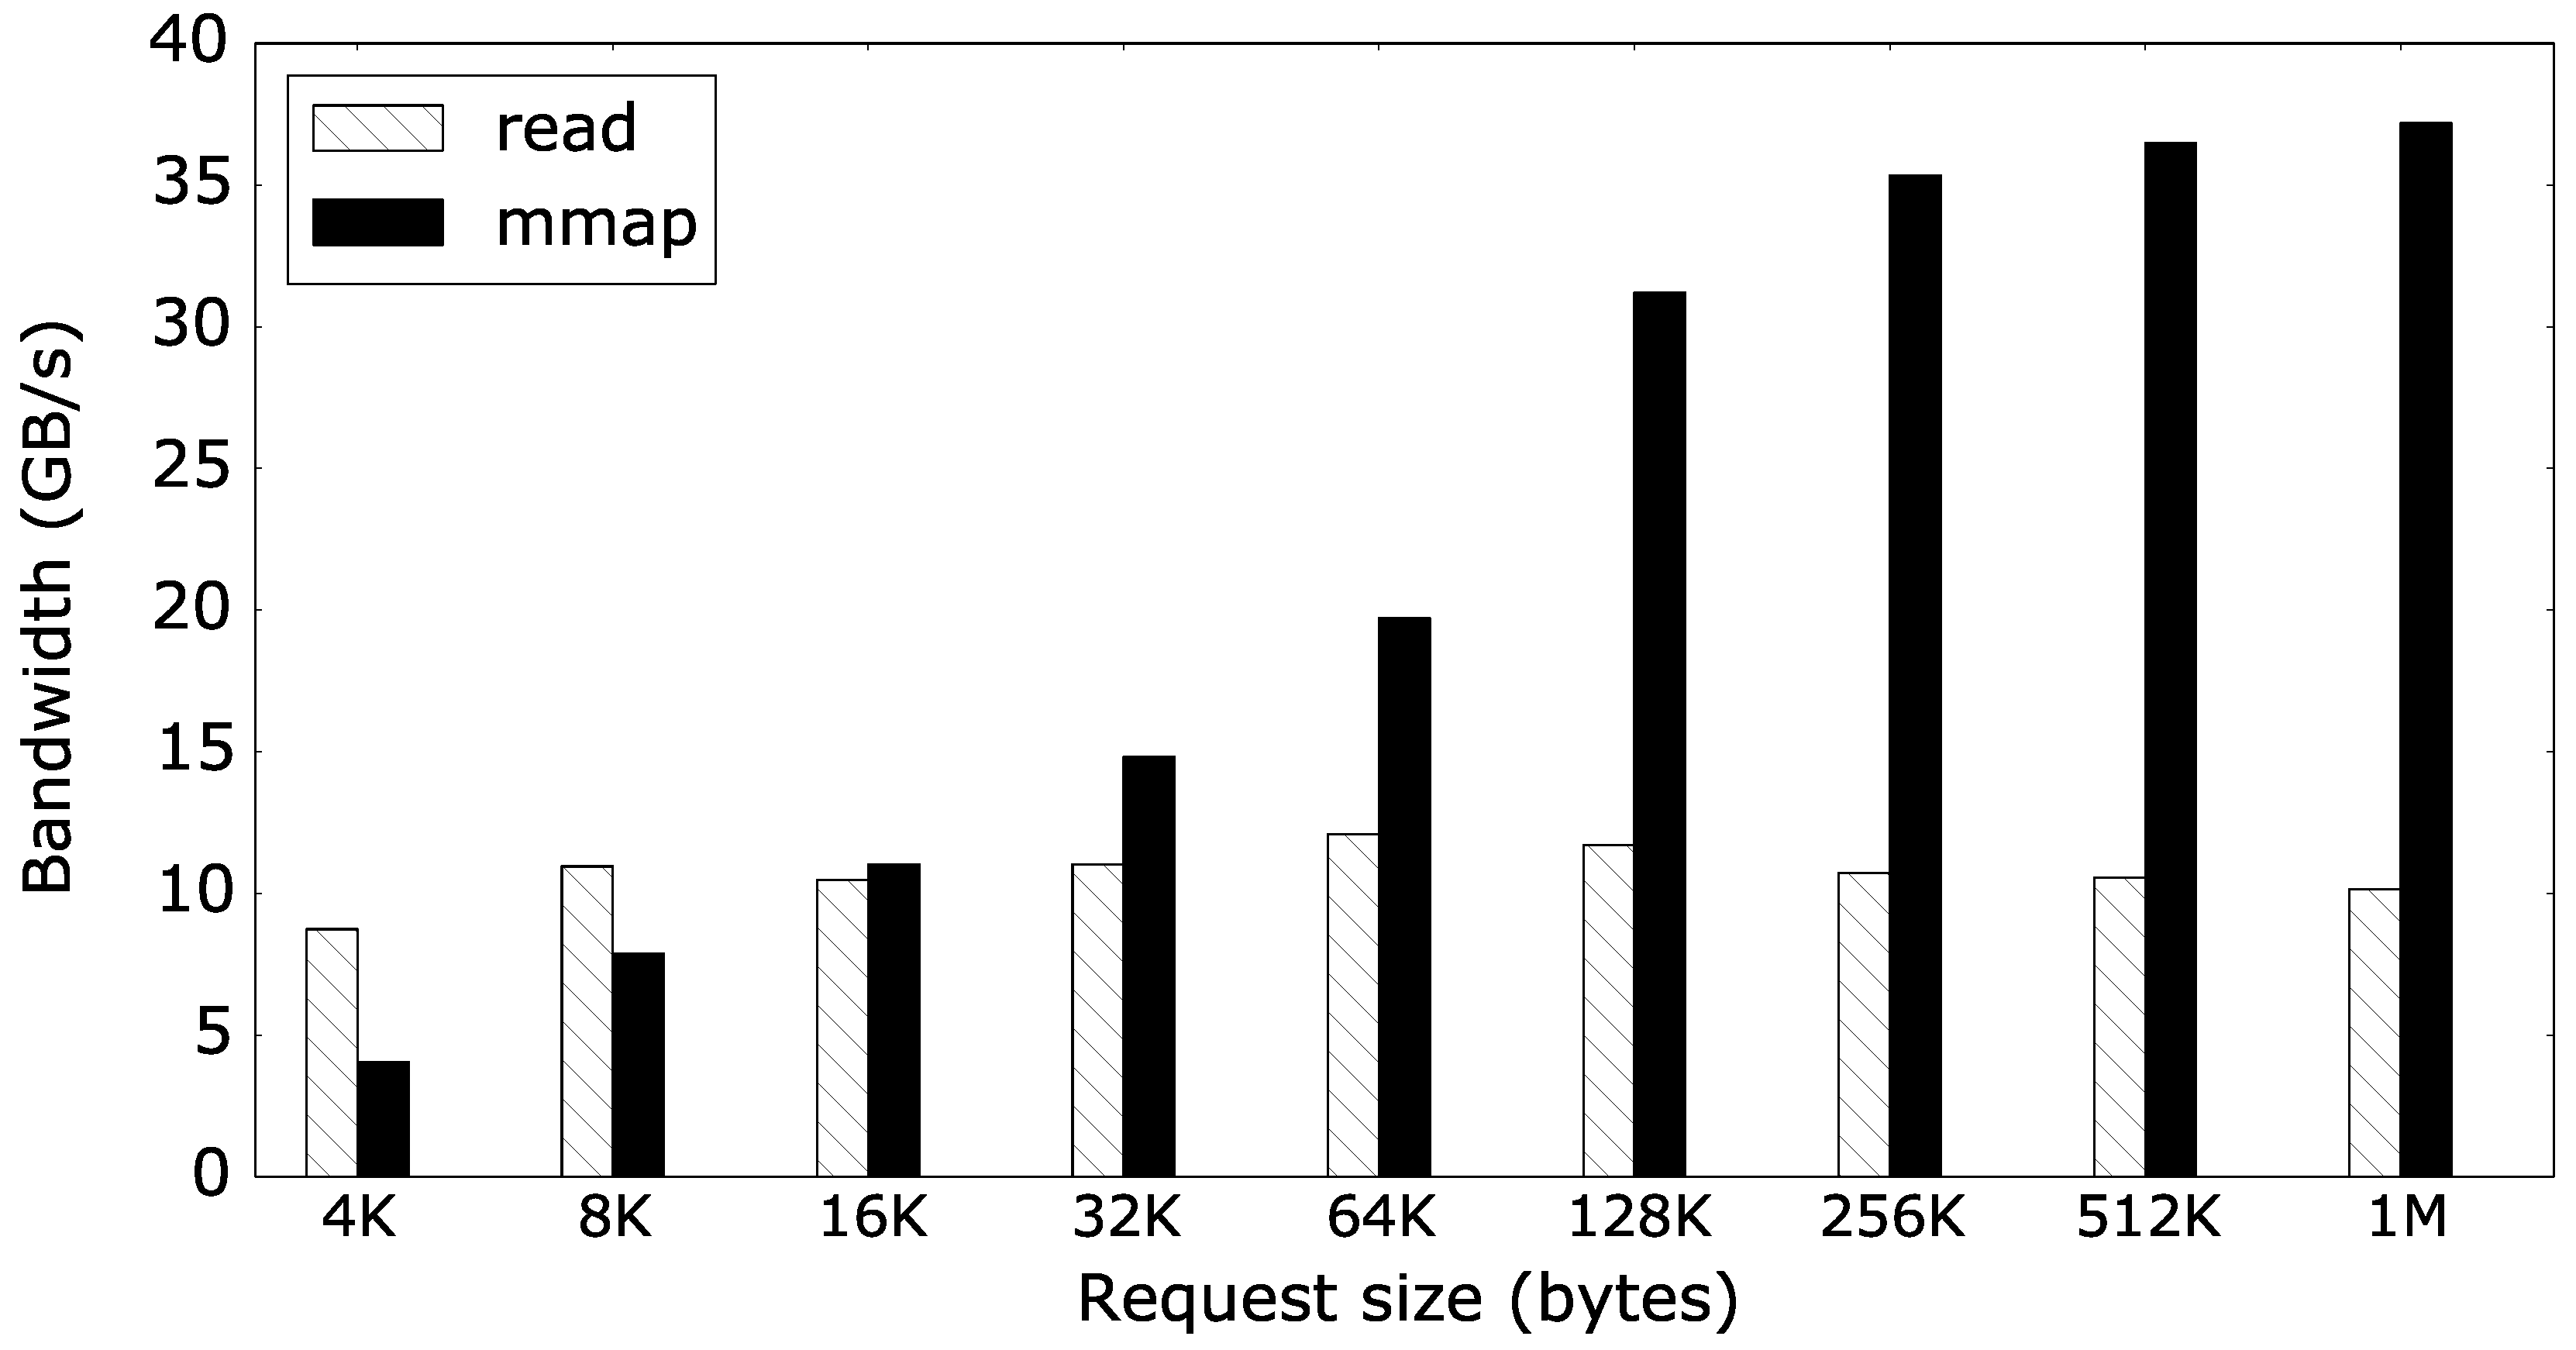
\includegraphics[width=\linewidth]{Graphs/mmap.pdf}
\caption{mmap performance}
\label{fig:mmap}
\end{figure}
}


\cfigure[Graphs/noposix.pdf,{\figtitle{\grb{} interface latency for different request sizes: latency of PMFS and \DAChell{} increases with request size, while \grb{} has constant latency}},fig:noposix]

\ignore{
Figure~\ref{fig:mmap} compares the performance of \grb{} and \texttt{read}
for files stored in NVMM with PMFS.  Conventional \andiry{\texttt{read} is faster for request sizes
below 8~kB WHy is this?}, but \grb{} outperforms \texttt{read} by up to 366\%. This is
because \grb{} calls \texttt{mmap()} for each request\andiry{why?}, for small
request the overhead of mmap operation (about 1000~ns) is larger than the
\texttt{memcpy} operation performed by \texttt{read} (about 400~ns for 4~kB) , but
for larger requests, the overhead of \grb{} is a
page fault to setup the persistent memory page in the page table
(about 100~ns), which is much smaller than a 4~kB \texttt{memcpy} of POSIX
read. \andiry{This seems like a pretty inefficient way to do this.  If the file is already in memory, for \DAChell{}, the latency for \grb{} should be just the lookup time in the btree}
}

Figure~\ref{fig:noposix} compares the performance of the normal POSIX interface
and \texttt{\grb{}} for a sequential read workload running on PMFS with
\Chell{} enabled.  The copy that the POSIX interface requires causes latency to
increase linearly with request size.  \texttt{\grb{}} does not do any copying, so
latency is nearly constant.  For 4~kB request, \grb{} outperforms POSIX for
4.2\x{}, and for 1~MB request, \texttt{\grb{}} achieves performance gain up to
700\x{}.


